%LaTeX
%\documentclass[twoside]{article}
\documentclass{article}
%This makes the margins little smaller than the default
%\usepackage{fullpage}
%fullpage is not installed on andrew, so we'll just use these lines.
\oddsidemargin0cm
\topmargin-2cm     %I recommend adding these three lines to increase the 
\textwidth16.5cm   %amount of usable space on the page (and save trees)
\textheight23.5cm  


%if you need more complicated math stuff, you should use the next line
%\usepackage{amsmath}
%This next line defines a variety of special math symbols which you
%may need
\usepackage{amssymb}

%This next line (when uncommented) allow you to use encapsulated
%postscript files for figures in your document
%\usepackage{epsfig}
\usepackage{graphicx}


%plain makes sure that we have page numbers
\pagestyle{plain}


\title{
        16-868F13: Biomechanics and Motor Control \linebreak
        Assignment 1
}
\author{
        Benjamin Shih (bshih1)
       }
\date{Start: Sept 8 2013 \linebreak
      End: Sept 17 2013
     }

%This defines a new command \questionhead which takes one argument and
%prints out Question #. with some space.
\newcommand{\questionhead}[1]
  {\bigskip\bigskip
   \noindent{\LARGE\bf Question #1}
   \bigskip}


%-----------------------------------
\begin{document}
%-----------------------------------

\maketitle


\questionhead{1}

\noindent{\Large Simulation: Develop a 2D simulation model of standing balance in SimMechanics (Fig. 1).}

\begin{center}
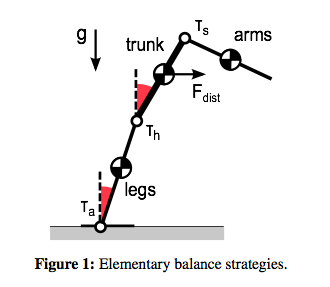
\includegraphics{fig1.png}
\end{center}

\noindent{\large a) First, implement the ankle strategy for a simple inverted pendulum model. Use SimMechanics to build this initial model which only represents the “legs segment” with length ll = 1m and mass ml = 20kg. The segment mass is concentrated in a point at half the segment length. Implement the ankle strategy as a torque τa generated by a PD control of the legs segment angle with respect to gravity. Measure the center of pressure (COP) and saturate the torque output if the COP exceeds an assumed horizontal foot range between -5cm to +20cm relative to the ankle.}\\

Using the foot-leg model provided with the assignment, I added a saturation limit for the torque output if the center of pressure (COP) exceeded an assumed horizontal foot range between -5cm and 20cm. The enable block is shown below:

\begin{center}
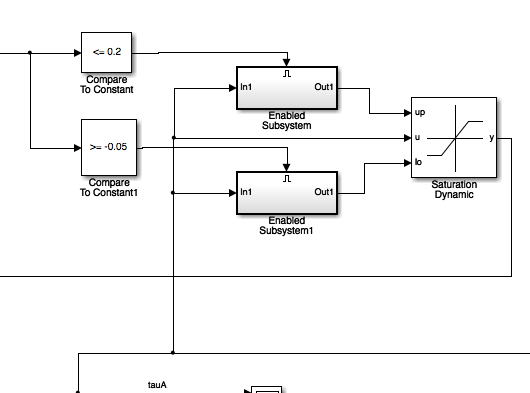
\includegraphics[scale=0.75]{1a_enable.png}
\end{center}

The resulting center of pressure convergence looks like:

\begin{center}
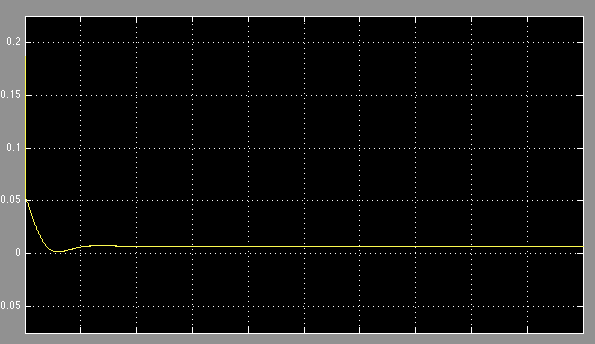
\includegraphics[scale=0.75]{1a_COP.png}
\end{center}

As a result of the torque saturation, the COP never exceeds the range of [-0.05, 0.2] m. The final leg simulation is shown below:

\begin{center}
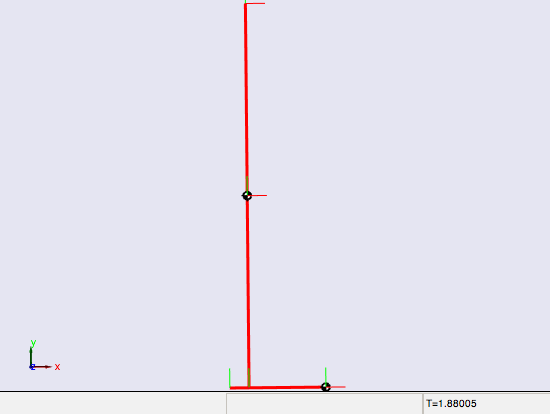
\includegraphics[scale=0.75]{1a_leg.png}
\end{center}

\noindent{\large b) Second, add a trunk segment. The trunk segment is 0.8m long and weighs 50kg (mass again concentrated at half segment length). The trunk is actuated via the hip torque τh by a PD control that tries to keep the trunk upright at all times. The maximum torque output is limited to 500Nm. Start with the legs and trunk in upright position and simulate balance disturbances by a horizon- tal force applied for 100ms at the trunk’s center of mass. Use the “body actuator” and “step function” elements of the SimMechanics and Simulink libraries to implement the disturbance force. Demonstrate a range of disturbances that can be compensated with this two segment system, and then some disturbances that cannot.}\\

I added the trunk segment by replicating the leg segment and modifying the physical parameters associated with the drunk, as well as the controller gains. The torque saturation was changed to a static saturation block that had limits of -500 and 500 Nm. The external disturbance force was implemented using a body actuator and a step function as follows:

\begin{center}
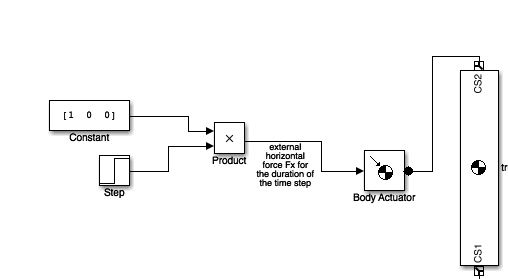
\includegraphics[scale=0.75]{1b_fx.png}
\end{center}


After testing, stability for an externally applied $F_x$ appears to range from 0 N (no applied external force) to +45 N. I would have expected the body to better withstand bigger forces in the +x direction because the center of mass of the foot is in front of the leg and trunk segments. However, when my leg is hit by a non-zero magnitude force in the -x direction, it appears to encounter right half plane poles in the system dynamics because the oscillation becomes unstable rather than converging. However, this could be solved in the future with further PD control gain-tuning. The final leg-trunk simulation is shown below:

\begin{center}
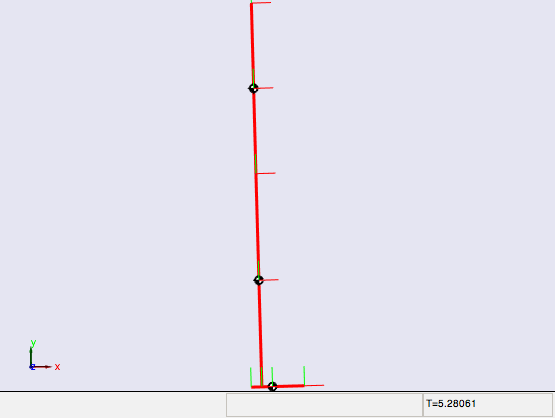
\includegraphics[scale=0.75]{1b_leg.png}
\end{center}

\noindent{\large c) Finally, implement the hip strategy using the “arms segment” as a flywheel. The segment’s mass and length are 5kg and 1m, respectively. The mass is concentrated at half the segment length. The maximum shoulder torque τs that can be applied is 50Nm. Repeat the disturbance experiments. What maximum disturbance forces can you now compensate in the forward and backward directions?}\\

In my model, the maximum disturbance forces decrease when the flywheel is added. However, given that the gains are properly selected, I would expect the maximum disturbance forces in both the forward and backward directions to increase because the arms acting as a flywheel allows the model to generate a counter-torque in order to balance any external disturbances. The error can be attributed to modifying the PD control gains, and stability can be achieved in the future by further tuning the gains. The final leg-trunk-arms simulation is shown below:

\begin{center}
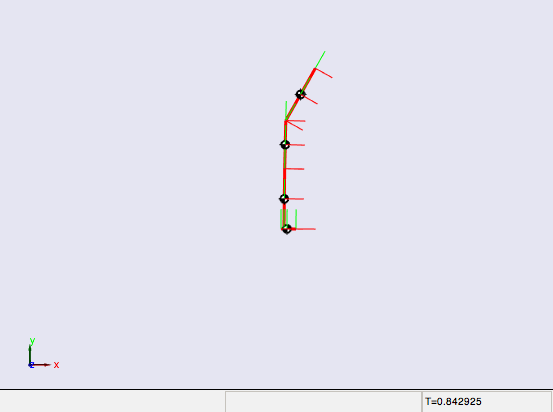
\includegraphics[scale=0.75]{1c_flywheel.png}
\end{center}


\noindent{\large d) What happens to the arms segment after the disturbances are over and how does this behavior compare to human behavior? Try to modify the balance control to better describe human behavior.}\\

After the disturbances are over, the arms settle to a resting position. This compares to human behavior because the scenario is analogous to how we balance ourselves when, for example, another person shoves us. Our arms act as flywheels to generate torque that counter-balances the externally applied force. However, once the external force is neutralized, the flywheel should stop generating torque and thus our arms come to a rest. In my simulation, tuning the gain allows me to better emulate the flywheel response that humans have when pushed. 




%%%%%%%%%%%%%%%%%%%%%%%%%%%%%%%%%%%%%%%%%%%%%%%%%%%%%%%%
\questionhead{2}

\noindent{\Large General Research Skills: The ankle strategy requires to estimate the center of pressure (COP). One hypothesis is that humans directly measure their COP. Conduct an independent literature search and find at least one study that supports or refutes this hypothesis.}\\
 
\emph{Motion sickness preceded by unstable displacements of the center of pressure} by Bonnet et. al. supports the hypothesis that humans directly measure their center of pressure (COP) in a manner similar to that observed in the ankle strategy.

The experimental setup induced motion sickness in standing participants via optical flow in a moving room by simulating the amplitude and frequency of standing sway. Instabilities in displacements of the center of pressure were identified, before the onset of subjective motion, in participants who became sick. 

The results demonstrate that humans directly measure COP, because the human body acknowledges instabilities in displacements of COP by self-inducing nausea and motion sickness. They also are consistent with the postural instability theory of motion sickness, and support the hypothesis that instability in the control of stance is a necessary and sufficient precursor to motion sickness.

%%%%%%%%%%%%%%%%%%%%%%%%%%%%%%%%%%%%%%%%%%%%%%%%%%%%%%%%
\questionhead{3}

\noindent{\Large Theory: Derive the capture point for the stepping strategy in 3D.}\\

\begin{center}
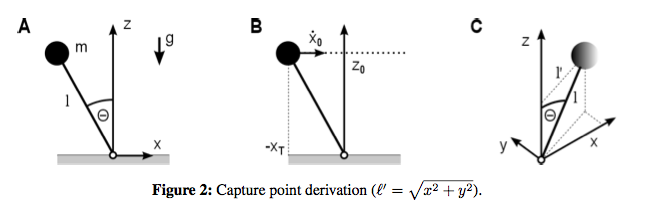
\includegraphics[scale=0.75]{fig2.png}
\end{center}

\noindent{\large a) Start with the inverted pendulum in 2D (Fig. 2A). Find the equation of motion for $\theta$ and then approximate it assuming $\theta \ll 1$. Now assume that instead of the leg length l, the vertical height stays constant, $z = z_0$, turning the model into the linear inverted pendulum. Given an initial velocity $\dot{x}_0$ that results from an unexpected push, derive the position $x_T$ where a humanoid leg needs to be placed to come to a rest at midstance (Fig. 2B). Hints: The first step result is $\ddot{x} - gx = 0$. Use the change in mechanical energy to find $x_T$.}\\

$\tau = I*\alpha$\\
$\rightarrow m*g*l*sin(\theta) = m*l^2*\theta$\\
By small angle approximation, for which $sin(\theta) \approx \theta$:\\
$\rightarrow m*g*\theta*l = m*\ddot{\theta}*l^2 $\\
$\leftrightarrow \ddot{\theta} - \frac{g}{l}*\theta = 0$\\
Again, by small angle approximation, $x \approx \theta, \ddot{x} \approx \ddot{\theta}, z  \approx l$:\\
$\rightarrow \ddot{x} - \frac{g}{z}*x = 0$\\

\noindent{\large b) Derive the capture point in 3D using the method developed for the 2D case. Figure 2C shows the inverted pendulum with constant leg length l in three-dimensional space. First identify the net forces that act in the x, y, and z direction. Then approximate the resulting equations of motion $m(\ddot{x}, \ddot{y}, \ddot{z})^T = (F_x,F_y,F_z)^T$ assuming Θ ≪ 1. Finally, make the transition to linear inverted pendulums and compute the capture point $(x_T,y_T)^T$ for an initial velocity($x_0, y_0)^T$. Hints: Only that part of the gravitational force vector which is perpendicular to the leg axis contributes to the net forces. You need to further decompose this part into its cartesian components. For example, the resulting force in z-direction is $F_z = mg sin^2(\theta)$. For small angles $\theta$, $\theta^2$ can be neglected.}\\

\begin{center}
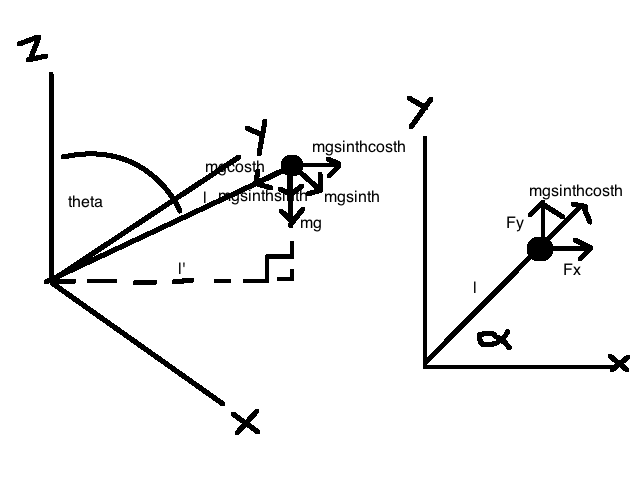
\includegraphics[scale=0.65]{3b_visual.png}
\end{center}


The horizontal force can be denoted as $F_H = m*g*sin(\theta)*cos(\theta)$. In order to obtain the components $F_x$ and $F_y$, we need to split up $F_H$ one more time using angle $\alpha$. By doing this, we see:

$\newline F_x = m*g*sin(\theta)*cos(\theta)*\frac{x}{\sqrt{x^2+y^2}}$\\
But, since $sin(\theta) = \frac{l'}{l}$:\\
$\newline \leftrightarrow F_x = m*g*\frac{l'}{l}*cos(\theta)*\frac{x}{\sqrt{x^2+y^2}}$\\
From the picture we can see that $l' = \sqrt{x^2+y^2}$, and by small angle approximation we can approximate $cos(\theta) \approx 1-\frac{\theta^2}{2}$, which is approximately 1 since for small angles $\theta^2$ can be neglected:\\
$\newline \rightarrow F_x = m*g*\frac{x}{l}$

$\newline F_y = m*g*\frac{y}{l}$ can be obtained in a similar fashion. 

$\newline$ Lastly, from earlier, $F_z = m*g*sin^2(\theta)$, which concludes our equations of motion.

$\newline$ In order to make the transition to linear inverted pendulum model, we assume that our leg length can change such that it is fixed at a height of $z_0$. 

$\newline \rightarrow F_x = m*g*\frac{x}{z_0}$

$\newline$ Using energy balance, we obtain:

$\newline \frac{m}{2}*\dot{x}_{0}^2 = \int_0^{x_T} m * g * \frac{x}{z_0} * dx$
$\newline \leftrightarrow \frac{m}{2}*\dot{x}_{0}^2 = \frac{m*g}{z_0}*\frac{x_T^2}{2}$
$\newline \leftrightarrow x_T = \sqrt{\frac{z_0}{g}}*\dot{x}_0$

$\newline y_T = \sqrt{\frac{z_0}{g}}*\dot{y}_0$ can be obtained in a similar fashion, which makes sense because the problem is symmetric about the z-axis. 

%-------------------------
\end{document}
%-------------------------







